%%%%%%%%%%%%%%%%%%%%%%%%%%%%%%%%%%%%%%%%%%%%%%%%%%%%%%%%%%%
%%%                                                     %%%
%%%   LaTeX template voor P&O: Computerwetenschappen.   %%%
%%%                                                     %%%
%%%   Schrijfopdracht 1                                 %%%
%%%                                                     %%%
%%%   7 oktober 2013                                    %%%
%%%   Versie 1.1                                        %%%
%%%                                                     %%%
%%%%%%%%%%%%%%%%%%%%%%%%%%%%%%%%%%%%%%%%%%%%%%%%%%%%%%%%%%%

\documentclass{peno-opdracht1}

\team{Indigo} % teamkleur

\begin{document}

\maketitle

Het doel van deze opdracht is een autonome zeppelin te ontwikkelen. De zeppelin wordt aangestuurd door een Raspberry Pi. Via QR-codes kunnen instructies gegeven worden, zoals ``stijg 50cm'' of ``draai 45   graden''. De gebruiker kan via een GUI op een client-pc zelf via de pijltjestoetsen de zeppelin aansturen of gegevens bekijken over de toestand van de zeppelin (bijvoorbeeld de huidige hoogte).

\paragraph{Fysisch ontwerp:}
~\\ 
De zeppelin bestaat uit een houten frame waaraan 2 grote ronde heliumballonnen vastgemaakt zijn. Aan het frame is een afstandssensor gekoppeld die naar onderen is gericht. Op het voorste deel van het frame hangt ook een camera die beelden maakt van de omgeving. Zowel de camera alsook de afstandssensor zijn verbonden met de Raspberry Pi die in het frame zit ingebed. Het geheel bevat drie propellers: twee voor zijwaartse bewegingen en \'{e}\'{e}n voor opwaartse bewegingen.


\paragraph{Software ontwerp:}
~\\
Natuurlijk moet de zeppelin aangestuurd worden via de software. Dit is onderverdeeld in 3 grote delen: de GUI, de communicatie tussen GUI en Raspberry Pi en de interne programmatie op de Pi (Zie figuur \ref{schema}). De software zal volledig worden geprogrammeerd in Java. 
De communicatie tussen GUI en de Raspberry Pi zal gebeuren via sockets. Hierbij worden objecten uitgewisseld tussen de client en de server (de Pi) die commando's doorgeven aan de zeppelin of de status doorgeven aan de gebruiker. De interne programmatie op de Pi moet op basis van zijn sensoren en commando's de motoren aansturen. 




\begin{figure}[ht!]
\centering
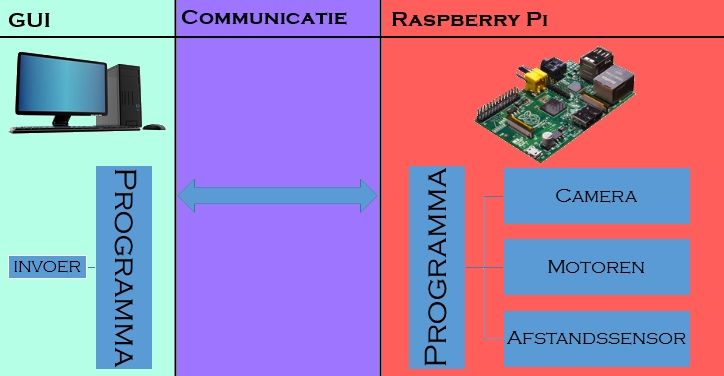
\includegraphics[height=55mm]{Schema.jpg}
\caption{Architectuur}
\label{schema}
\end{figure}






\end{document}
